 \documentclass[9pt]{beamer}
%\documentclass[compress,9pt,usenames,dvipsnames]{beamer}
% \usepackage[utf8]{inputenc}
% \includeonlyframes{current}
\setbeamercovered{dynamic}
\usepackage{etex}
\usepackage{graphicx,url,psfrag}
\usepackage{tikz}
\usetikzlibrary{decorations.pathreplacing,calc,decorations.fractals,through,shapes,patterns,arrows.meta,decorations.pathreplacing,arrows,shapes,}
\usepackage{tikzpeople}
% \usepackage[center]{subfigure}
\usepackage{enumerate}
\usepackage[makeroom]{cancel}
\usepackage{mathtools}
\usepackage{graphbox}
\usepackage{amssymb}
\usepackage{comment}
\excludecomment{codes}
% \usepackage{movie15}
% \usepackage[showframe]{geometry}
% \usepackage{enumitem}

%
% for warning sign
%
\usepackage{pgfplots}
\usepackage{stackengine}
\usepackage{scalerel}
\usepackage{xcolor}
\usepackage{dbt}
\newcommand\dangersign[1][2ex]{%
  \renewcommand\stacktype{L}%
  \scaleto{\stackon[1.3pt]{\color{red}$\triangle$}{\tiny !}}{#1}%
}
% %  The following is to show codes:
\usepackage{listings}
% \usepackage{color}

\usepackage{pifont}% http://ctan.org/pkg/pifont
\newcommand{\cmark}{\ding{51}}%
\newcommand{\xmark}{\ding{55}}%

\definecolor{dkgreen}{rgb}{0,0.6,0}
\definecolor{gray}{rgb}{0.5,0.5,0.5}
\definecolor{mauve}{rgb}{0.58,0,0.82}

\lstset{frame=tb,
  language=Java,
  aboveskip=3mm,
  belowskip=3mm,
  showstringspaces=false,
  columns=flexible,
  basicstyle={\small\ttfamily},
  numbers=none,
  numberstyle=\tiny\color{gray},
  keywordstyle=\color{blue},
  commentstyle=\color{dkgreen},
  stringstyle=\color{mauve},
  breaklines=true,
  breakatwhitespace=true,
  tabsize=3
}
\lstset{language=Python}

\lstset{ %
  language=Python,                     % the language of the code
  basicstyle=\footnotesize,       % the size of the fonts that are used for the code
  numbers=left,                   % where to put the line-numbers
  numberstyle=\tiny\color{gray},  % the style that is used for the line-numbers
  stepnumber=1,                   % the step between two line-numbers. If it's 1, each line
                                  % will be numbered
  numbersep=5pt,                  % how far the line-numbers are from the code
  backgroundcolor=\color{black},  % choose the background color. You must add \usepackage{color}
  showspaces=false,               % show spaces adding particular underscores
  showstringspaces=false,         % underline spaces within strings
  showtabs=false,                 % show tabs within strings adding particular underscores
  frame=single,                   % adds a frame around the code
  rulecolor=\color{black},        % if not set, the frame-color may be changed on line-breaks within not-black text (e.g. commens (green here))
  tabsize=2,                      % sets default tabsize to 2 spaces
  captionpos=b,                   % sets the caption-position to bottom
  breaklines=true,                % sets automatic line breaking
  breakatwhitespace=false,        % sets if automatic breaks should only happen at whitespace
  title=\lstname,                 % show the filename of files included with \lstinputlisting;
                                  % also try caption instead of title
  keywordstyle=\color{blue},      % keyword style
  commentstyle=\color{dkgreen},   % comment style
  stringstyle=\color{mauve},      % string literal style
  escapeinside={\%*}{*)},         % if you want to add a comment within your code
  morekeywords={*,...}            % if you want to add more keywords to the set
}
% \usepackage[usenames,dvipsnames]{color}
% \lstset{
%   language=R,                     % the language of the code
%   basicstyle=\tiny\ttfamily, % the size of the fonts that are used for the code
%   numbers=left,                   % where to put the line-numbers
%   numberstyle=\tiny\color{Blue},  % the style that is used for the line-numbers
%   stepnumber=1,                   % the step between two line-numbers. If it is 1, each line
%                                   % will be numbered
%   numbersep=5pt,                  % how far the line-numbers are from the code
%   backgroundcolor=\color{white},  % choose the background color. You must add \usepackage{color}
%   showspaces=false,               % show spaces adding particular underscores
%   showstringspaces=false,         % underline spaces within strings
%   showtabs=false,                 % show tabs within strings adding particular underscores
%   frame=single,                   % adds a frame around the code
%   rulecolor=\color{black},        % if not set, the frame-color may be changed on line-breaks within not-black text (e.g. commens (green here))
%   tabsize=2,                      % sets default tabsize to 2 spaces
%   captionpos=b,                   % sets the caption-position to bottom
%   breaklines=true,                % sets automatic line breaking
%   breakatwhitespace=false,        % sets if automatic breaks should only happen at whitespace
%   keywordstyle=\color{RoyalBlue},      % keyword style
%   commentstyle=\color{YellowGreen},   % comment style
%   stringstyle=\color{ForestGreen}      % string literal style
% }

% \usepackage[dvipsnames]{xcolor}
% \newcommand{\Cross}{\mathbin{\tikz [x=1.4ex,y=1.4ex,line width=.2ex] \draw (0,0) -- (1,1) (0,1) -- (1,0);}}%
\newcommand{\Crossme}[1]{\!\!
\tikz [black,x=1.1em,y=1.1em,line width=.4ex]
\draw (-0.5,-0.5) -- (0,0) node {\footnotesize #1} -- (0.5,0.5) (0.5,-0.5) -- (-0.5,0.5);}%
\newcommand{\Checkme}[1]{\!\!
\tikz [x=1.1em,y=1.1em,line width=.4ex]
\draw [black] (0,0.7) -- (0.3,0) --(0.9,1.0) (0.5,0.5) node {\footnotesize #1};}
% \beamerdefaultoverlayspecification{<+-| alert@+>} %(this will show line by line)
\beamerdefaultoverlayspecification{<+->} %(this will show line by

% \usepackage{natbib}
% \input{../myMathSymbols.tex}
% \newcommand{\tlMr}[4]{\:{}^{\hspace{0.2em}#1}_{#2} \hspace{-0.1em}#3_{#4}}

% Smiley face\Smiley{} \Frowny{}
\usepackage{marvosym}
% -------------------------------------------------
%  Set directory for figs
% -------------------------------------------------
\usepackage{grffile}
\graphicspath{{Codes/}}
% -------------------------------------------------
%  Define colors
% -------------------------------------------------
\def\refcolor{cyan}
\def\excolor{brown}
% \usepackage{color}
% \usepackage[dvipsnames]{xcolor}


% % % Define danger sign
\newcommand*{\TakeFourierOrnament}[1]{{%
\fontencoding{U}\fontfamily{futs}\selectfont\char#1}}
\newcommand*{\danger}{\TakeFourierOrnament{66}}


% -------------------------------------------------
%  Define short-hand symbols.
% -------------------------------------------------
\newcommand{\B}{\textbf{B}}
\newcommand{\PP}{\mathbb{P}}
\newcommand{\E}{\mathbb{E}}
\newcommand{\D}{\mathbb{D}}
\newcommand{\W}{\dot{W}}
\newcommand{\ud}{\ensuremath{\mathrm{d}}}
\newcommand{\Ceil}[1]{\left\lceil #1 \right\rceil}
\newcommand{\Floor}[1]{\left\lfloor #1 \right\rfloor}
\newcommand{\sgn}{\text{sgn}}
\newcommand{\Lad}{\text{L}_{\text{ad}}^2}
\newcommand{\SI}[1]{\mathcal{I}\left[#1 \right]}
\newcommand{\SIB}[2]{\mathcal{I}_{#2}\left[#1 \right]}
\newcommand{\Indt}[1]{1_{\left\{#1 \right\}}}
\newcommand{\LadInPrd}[1]{\left\langle #1 \right\rangle_{\text{L}_\text{ad}^2}}
\newcommand{\LadNorm}[1]{\left|\left|  #1 \right|\right|_{\text{L}_\text{ad}^2}}
\newcommand{\Norm}[1]{\left|\left|  #1   \right|\right|}
\newcommand{\Ito}{It\^{o} }
\newcommand{\Itos}{It\^{o}'s }
\newcommand{\spt}[1]{\text{supp}\left(#1\right)}
\newcommand{\InPrd}[1]{\left\langle #1 \right\rangle}
\newcommand{\mr}{\textbf{r}}
\newcommand{\Ei}{\text{Ei}}
\newcommand{\arctanh}{\operatorname{arctanh}}
\newcommand{\ind}[1]{\mathbb{I}_{\left\{ {#1} \right\} }}
\newcommand{\Var}{\text{Var}}
\newcommand{\Cov}{\text{Cov}}
\newcommand{\Corr}{\text{Corr}}

\newcommand{\baseurl}[1]{\footnotesize\url{http://math.emory.edu/~lchen41/teaching/2020_Spring/#1}}


\newcommand*\mystrut[1]{\vrule width0pt height0pt depth#1\relax} % adding vertical space

\DeclareMathOperator{\esssup}{\ensuremath{ess\,sup}}

\newcommand{\steps}[1]{\vskip 0.3cm \textbf{#1}}
\newcommand{\calB}{\mathcal{B}}
\newcommand{\calC}{\mathcal{C}}
\newcommand{\calD}{\mathcal{D}}
\newcommand{\calE}{\mathcal{E}}
\newcommand{\calF}{\mathcal{F}}
\newcommand{\calG}{\mathcal{G}}
\newcommand{\calK}{\mathcal{K}}
\newcommand{\calH}{\mathcal{H}}
\newcommand{\calI}{\mathcal{I}}
\newcommand{\calL}{\mathcal{L}}
\newcommand{\calM}{\mathcal{M}}
\newcommand{\calN}{\mathcal{N}}
\newcommand{\calO}{\mathcal{O}}
\newcommand{\calT}{\mathcal{T}}
\newcommand{\calP}{\mathcal{P}}
\newcommand{\calR}{\mathcal{R}}
\newcommand{\calS}{\mathcal{S}}
\newcommand{\calV}{\mathcal{V}}
\newcommand{\bbC}{\mathbb{C}}
\newcommand{\bbN}{\mathbb{N}}
\newcommand{\bbP}{\mathbb{P}}
\newcommand{\bbZ}{\mathbb{Z}}
\newcommand{\myVec}[1]{\overrightarrow{#1}}
\newcommand{\sincos}{\begin{array}{c} \cos \\ \sin \end{array}\!\!}
\newcommand{\CvBc}[1]{\left\{\:#1\:\right\}}
\newcommand*{\one}{{{\rm 1\mkern-1.5mu}\!{\rm I}}}

\newcommand{\OneFrame}[1]{
\begin{enumerate}\item[#1] \phantom{av} \\[20em]\vfill\phantom{av}\myEnd\end{enumerate}}

\newcommand{\bH}{\ensuremath{\mathrm{H}}}
\newcommand{\Ai}{\ensuremath{\mathrm{Ai}}}

\newcommand{\R}{\mathbb{R}}
\newcommand{\myEnd}{\hfill$\square$}
\newcommand{\ds}{\displaystyle}
\newcommand{\Shi}{\text{Shi}}
\newcommand{\Chi}{\text{Chi}}
\newcommand{\Erf}{\ensuremath{\mathrm{erf}}}
\newcommand{\Erfc}{\ensuremath{\mathrm{erfc}}}
\newcommand{\He}{\ensuremath{\mathrm{He}}}
\newcommand{\Res}{\ensuremath{\mathrm{Res}}}

\newcommand{\mySeparateLine}{\begin{center}
 \makebox[\linewidth]{\rule{0.6\paperwidth}{0.4pt}}
\end{center}}

\theoremstyle{definition}
% \newtheorem{definition}[theorem]{Definition}
% \newtheorem{hypothesis}[theorem]{Hypothesis}
\newtheorem{assumption}[theorem]{Assumption}

\theoremstyle{plain}
% \newtheorem{theorem}{Theorem}
% \newtheorem{corollary}[theorem]{Corollary}
% \newtheorem{lemma}[theorem]{Lemma}
\newtheorem{proposition}[theorem]{Proposition}

\mode<presentation>
{
%      \usetheme{Warsaw}
%     \usetheme{JuanLesPins}
%  \usetheme{Hannover}
%  \usetheme{Montpellier}
   \useoutertheme{default}
  % or ...

  \setbeamercovered{transparent}
  % or whatever (possibly just delete it)
 \setbeamertemplate{frametitle}{
  \begin{centering}
    \color{blue}
    {\insertframetitle}
    \par
  \end{centering}
  }
}
\usefoottemplate{\hfill \insertframenumber{}}
% \inserttotalframenumber

\usepackage[english]{babel}
% or whatever

% \usepackage[latin1]{inputenc}
% or whatever

\usepackage{times}
\usepackage[T1]{fontenc}
% Or whatever. Note that the encoding and the font should match. If T1
% does not look nice, try deleting the line with the fontenc.

% \DeclareMathOperator{\Lip}{Lip}
\DeclareMathOperator{\lip}{l}
% \DeclareMathOperator{\Vip}{\overline{v}}
% \DeclareMathOperator{\vip}{\underline{v}}
% \DeclareMathOperator{\vv}{v}
% \DeclareMathOperator{\BC}{BC}
% \DeclareMathOperator{\CH}{CD}

\usepackage{pgfpages}
% \setbeameroption{show notes}
% \setbeamertemplate{note page}[plain]
% \setbeameroption{second mode text on second screen=right}
% \setbeameroption{show notes on second screen=right}
%

% Delete this, if you do not want the table of contents to pop up at
% the beginning of each subsection:
% \AtBeginSubsection[]
% {
%   \begin{frame}<beamer>{Outline}
%     \tableofcontents[currentsection,currentsubsection]
%   \end{frame}
% }

% If you wish to uncover everything in a step-wise fashion, uncomment
% the following command:
% \beamerdefaultoverlayspecification{<+->}

% % % % % % % % % % % % % % % % % % %
%  Define a block
% % % % % % % % % % % % % % % % % % %
\newenvironment<>{problock}[1]{%
  \begin{actionenv}#2%
      \def\insertblocktitle{#1}%
      \par%
      \mode<presentation>{%
        \setbeamercolor{block title}{fg=white,bg=olive!95!black}
       \setbeamercolor{block body}{fg=black,bg=olive!25!white}
       \setbeamercolor{itemize item}{fg=white!20!white}
       \setbeamertemplate{itemize item}[triangle]
     }%
      \usebeamertemplate{block begin}}
    {\par\usebeamertemplate{block end}\end{actionenv}}

\newenvironment<>{assblock}[1]{%
  \begin{actionenv}#2%
      \def\insertblocktitle{#1}%
      \par%
      \mode<presentation>{%
        \setbeamercolor{block title}{fg=white,bg=green!50!black}
       \setbeamercolor{block body}{fg=black,bg=green!10}
       \setbeamercolor{itemize item}{fg=green!80!black}
       \setbeamertemplate{itemize item}[triangle]
     }%
      \usebeamertemplate{block begin}}
    {\par\usebeamertemplate{block end}\end{actionenv}}


% \newtheorem{proofnoend}{Proof.}
% \AtBeginEnvironment{proofnoend}{%
%   \setbeamercolor{block title}{use=example text,fg=lgtblue,bg=background}
%   % \setbeamercolor{block body}{parent=normal text,use=block title example,fg=yellow}
% }

% Define some colors
\definecolor{white}{HTML}{FFFFFF}              % #FFFFFF
\definecolor{pink}{HTML}{FB73BE}               % #FB73BE
\definecolor{coral}{HTML}{FF8D71}              % #FF8D71
\definecolor{yellow}{HTML}{FFE066}             % #FFE066
\definecolor{teal}{HTML}{59F3CE}               % #59F3CE
\definecolor{lgtblue}{HTML}{65D0FA} 	       % #65D0FA
\definecolor{blue}{HTML}{4984F2}               % #4984F2
\definecolor{purple}{HTML}{A87DFF}             % #A87DFF
\definecolor{red}{HTML}{FF3d30}                % #FF3d30
% \definecolor{magenta}{HTML}{FF80FF}                % #FF3d30
\definecolor{green}{HTML}{BBFFB9}              % #BBFFB9
% \definecolor{green}{HTML}{59F3CE}              % #BBFFB9
\setbeamercolor{alerted text}{fg=red}
% \setbeamercolor{block title}{bg=background,fg=lgtblue}

\setbeamercolor{section in toc}{fg=yellow}
\setbeamercolor{subsection in toc}{fg=red}

% \newtheorem{myexample}{\it Example}[section]
\newcounter{myexample}[section]
\resetcounteronoverlays{myexample}
\newenvironment{myexample}[1][]{\refstepcounter{myexample}\par\medskip
\noindent \textbf{\textcolor{green}{Example~\mySecNum-\themyexample~#1}} \rmfamily}{\medskip}

\newcounter{mydefinition}[section]
\resetcounteronoverlays{mydefinition}
\newenvironment{mydefinition}[1][]{\refstepcounter{mydefinition}\par\medskip
\noindent \textbf{\textcolor{yellow}{Definition~\mySecNum-\themydefinition~#1}} \rmfamily}{\medskip}

% \NewCommandCopy{\oldref}{\ref}
% \let\oldref\ref
\newcommand{\myref}[1]{\mySecNum-\ref{#1}}

\newcounter{remark}[section]
\resetcounteronoverlays{remark}
\newenvironment{remark}[1][]{\refstepcounter{remark}\par\medskip
\noindent \textbf{\textcolor{blue}{Remark~\mySecNum-\theremark~#1}} \rmfamily}{\medskip}

\newcounter{mythm}[section]
\resetcounteronoverlays{mythm}
\newenvironment{mythm}[1][]{\refstepcounter{mythm}\par\medskip
\noindent \textbf{\textcolor{lgtblue}{Theorem~\mySecNum-\themythm~#1}} \rmfamily}{\medskip}

\newenvironment{mycor}[1][]{\refstepcounter{mythm}\par\medskip
\noindent \textbf{\textcolor{lgtblue}{Corollary~\mySecNum-\themythm~#1}} \rmfamily}{\medskip}

% \newtheorem{solution}{\textcolor{purple}{Solution}}
\newenvironment{mysol}[1][]{\par\medskip
\noindent \textbf{\textcolor{purple}{Solution#1.~}} \rmfamily}{\medskip}

\newenvironment{myproof}[1][]{\par\medskip
\noindent \textbf{\textcolor{purple}{Proof#1.~}} \rmfamily}{\medskip}

\long\def\script#1{}

% \numberwithin{equation}{section}

% If you have a file called "university-logo-filename.xxx", where xxx
% is a graphic format that can be processed by latex or pdflatex,
% resp., then you can add a logo as follows:

% \pgfdeclareimage[height=1cm]{Emory}{figs/Emory.png}


\title % (optional, use only with long paper titles)
{
  Financial Mathematics \\
  \bigskip
  \small MATH 5870/6870\footnote{\textcolor{gray}{Based on Robert L. McDonald's {\it Derivatives Markets}, 3rd Ed, Pearson, 2013.}}\\
  Fall 2021
}

% \subtitle
% {Research Plan} % (optional)

\author{Le Chen\\[1em]
  {\small\textcolor{gray}{\url{lzc0090@auburn.edu}}}
}


\institute[Auburn University]
{
% \pgfuseimage{Emory}\\[3em]
% {\small Auburn University}\\[1em]
% {\small Auburn AL}\\[3em]
\textcolor{gray}{Last updated on } \\[1em]
\textcolor{gray}{\today}
 \vspace{8em}
}
% - Use the \inst command only if there are several affiliations.
% - Keep it simple, no one is interested in your street address.

\date[Auburn]{Auburn University\\ \textcolor{gray}{Auburn AL}}
% \date{}

% \subject{}



\begin{document}
\begin{frame}[noframenumbering]
  \titlepage
\end{frame}
\newcommand{\myChapter}{Chapter 3. Insurance, Collars, and Other Strategies}
\newcommand{\mySection}[1]{
  \section{\S\: #1}
  \begin{frame}{\myChapter}\tableofcontents\end{frame}
  \begin{frame}{\myChapter}\tableofcontents[currentsection]\end{frame}
  }
\begin{frame}
\begin{center}
\huge
\myChapter
\end{center}
\end{frame}
\def\mySecNum{3.1}
\mySection{\mySecNum~Basic insurance strategies}
%-------------- start slide -------------------------------%{{{ 1
\begin{frame}[fragile]
	Options can be
	\begin{enumerate}
		\item Used to insure long positions (floors)
		\item Used to insure short positions (caps)
		\item Written against asset positions (selling insurance)
		\item[] Covered call writing
		\item[] Covered put writing
	\end{enumerate}
\end{frame}
%-------------- end slide -------------------------------%}}}
%-------------- start slide -------------------------------%{{{ 1
\begin{frame}[fragile,t]
	\begin{center}
		Four positions
		\bigskip

		\renewcommand{\arraystretch}{1.2}
		\begin{tabular}{|c|c c|}
			\hline
			positions w.r.t. asset & put option                             & call option                       \\ \hline
			long                   & purchased (\textcolor{magenta}{floor}) & written                           \\
			short                  & written                                & purchased (\textcolor{cyan}{cap}) \\ \hline
		\end{tabular}
	\end{center}

	\bigskip
	\mySeparateLine
	\bigskip
	\begin{center}
		\begin{minipage}{0.45\textwidth}
			\centering
			Buying insurance
			\begin{align*}
				\textcolor{magenta}{floor} & = \text{buying a \textcolor{magenta}{put} option} \\
				\textcolor{cyan}{cap}      & = \text{buying a \textcolor{cyan}{call} option}
			\end{align*}
		\end{minipage}
		\begin{minipage}{0.3\textwidth}
			\centering
			Selling insurance
			\begin{align*}
				\text{Covered \textcolor{magenta}{put} writing} \\
				\text{Covered \textcolor{cyan}{call} writing}
			\end{align*}
		\end{minipage}
	\end{center}
\end{frame}
%-------------- end slide -------------------------------%}}}
%-------------- start slide -------------------------------%{{{ 1
\begin{frame}[fragile,t]
\begin{center}
	We will work under the following setup
	\bigskip
	\bigskip

	S\&S index\\
	\bigskip

	\renewcommand{\arraystretch}{1.2}
	\begin{tabular}{|c|c|}
		\hline
		index price today                                         & \$1,000  \\
    6-month interest rate                                     & 2\%      \\
		premium for 1000-strike 6-month \textcolor{magenta}{call} & \$93.809 \\
		premium for 1000-strike 6-month \textcolor{cyan}{put}     & \$74.201 \\ \hline
	\end{tabular}

\end{center}

\end{frame}
%-------------- end slide -------------------------------%}}}
%-------------- start slide -------------------------------%{{{ 1
\begin{frame}[fragile]
	\frametitle{Insuring a long position \\ -- \textcolor{magenta}{Floors}}

	\begin{center}
		\renewcommand{\arraystretch}{1.2}
		\begin{tabular}{|c|c|}
			owning a home      & owning a stock index                      \\
			insuring the house & buying a put (\textcolor{magenta}{floor}) \\
		\end{tabular}
		\bigskip
		\bigskip

		Goal: to insure against a fall in the price of the underlying asset.
	\end{center}

\end{frame}
%-------------- end slide -------------------------------%}}}
%-------------- start slide -------------------------------%{{{ 1
\begin{frame}[fragile]
	\begin{myexample}
		Under the following scenario, compute the combined profit of \underline{insuring a long
		position via \textcolor{cyan}{buying a put}} for the following S\&R index.
	\begin{center}
		\renewcommand{\arraystretch}{1.2}
		\begin{tabular}{|c|c|}
			\hline
			index price today                                     & \$1,000  \\
			6-month interest rate                                 & 2\%      \\
			% premium for 1000-strike 6-month call & \$93.809 \\ \hline
			premium for 1000-strike 6-month \textcolor{cyan}{put} & \$74.201 \\ \hline
			index price at expiration                             & \$900    \\ \hline
		\end{tabular}
	\end{center}
	\end{myexample}
	\vfill
	\pause
	\begin{mysol}
		\begin{align*}
			\underbrace{\$900 - \$1,000 \times 1.02}_{\text{profit on S\&R index}} +
			\underbrace{\$1,000-\$900 -\$74.201 \times 1.02}_{\text{profit on put}} = -\$95.68.
		\end{align*}
		\myEnd
	\end{mysol}
\end{frame}
%-------------- end slide -------------------------------%}}}
%-------------- start slide -------------------------------%{{{ 1
\begin{frame}[fragile,t]
	\begin{center}
		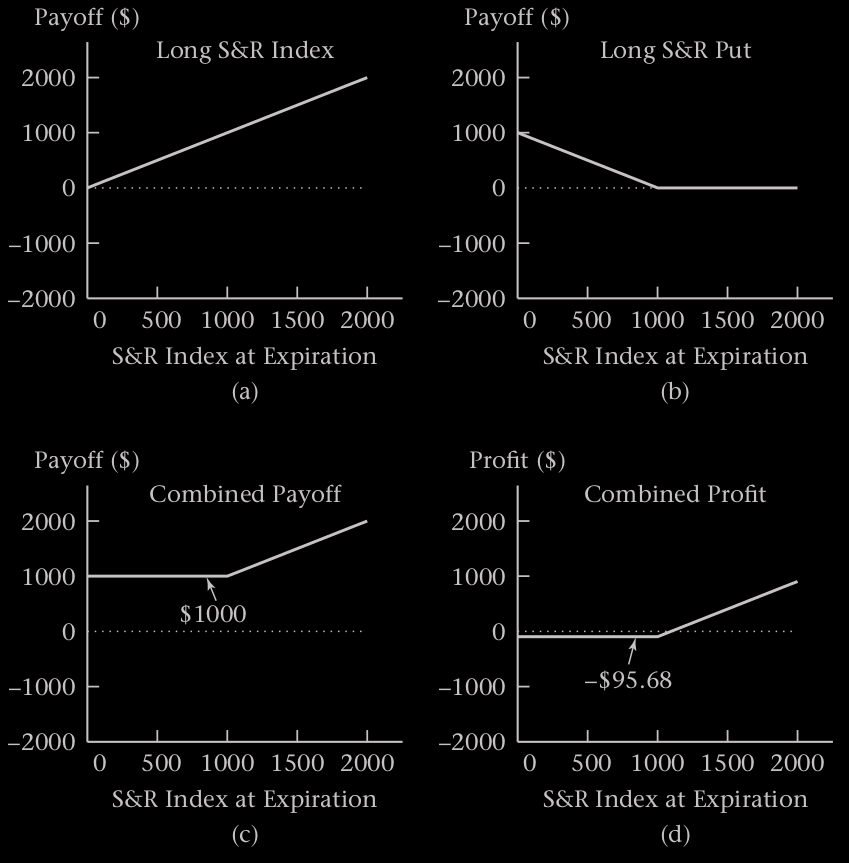
\includegraphics[scale=0.25]{figs/Figure-3-1.png}
	\end{center}
\end{frame}
%-------------- end slide -------------------------------%}}}
%-------------- start slide -------------------------------%{{{ 1
\begin{frame}[fragile]
\begin{center}
	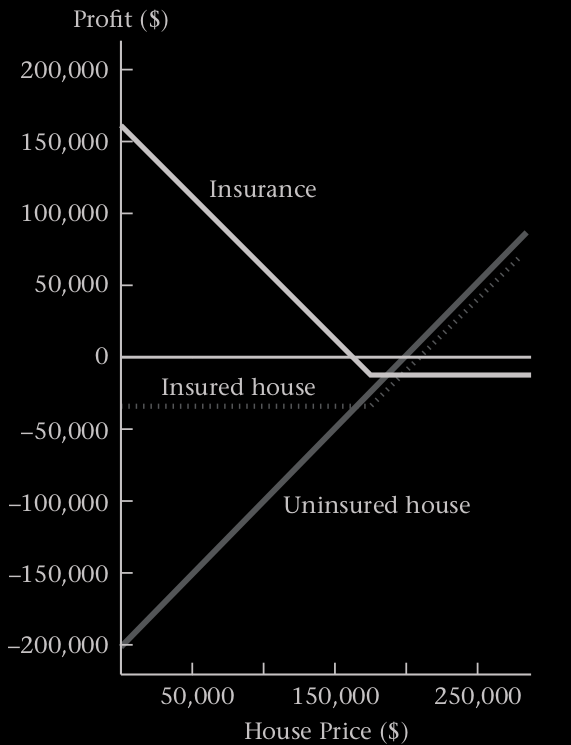
\includegraphics[scale=0.2]{figs/Figure-3-2.png}
\end{center}
\end{frame}
%-------------- end slide -------------------------------%}}}
%-------------- start slide -------------------------------%{{{ 1
\begin{frame}[fragile,t]
	\frametitle{Insuring a short position \\ -- \textcolor{magenta}{Caps}}

If we have a short position in the S\&R index, we experience a loss when the index rises.
\bigskip

We can insure a short position by \textcolor{cyan}{purchasing a call option (cap)} to protect against a
higher price of repurchasing the index.

\end{frame}
%-------------- end slide -------------------------------%}}}
%-------------- start slide -------------------------------%{{{ 1
\begin{frame}[fragile]
	\begin{myexample}
		Under the following scenario, compute the combined profit for \underline{insuring a short
		position via \textcolor{magenta}{buying a call}} of the following S\&R index.

		\begin{center}
			\renewcommand{\arraystretch}{1.2}
			\begin{tabular}{|c|c|}
				\hline
				index price today                                         & \$1,000  \\
				6-month interest rate                                     & 2\%      \\
				premium for 1000-strike 6-month \textcolor{magenta}{call} & \$93.809 \\ \hline
				% premium for 1000-strike 6-month put & \$74.201 \\ \hline
				index price at expiration                                 & \$1,100  \\ \hline
			\end{tabular}
		\end{center}
	\end{myexample}
	\vfill
	\pause
	\begin{mysol}
		\begin{align*}
			\underbrace{\$1,000 \times 1.02}_{\text{future value of short S\&R index}} - \: \:
			\underbrace{\$93.809 \times 1.02}_{\text{FV of premium for call}} - \:\:
			\underbrace{\$1,000}_{\text{exercise the call option}}
			= -\$75.685.
		\end{align*}
		\myEnd
	\end{mysol}
\end{frame}
%-------------- end slide -------------------------------%}}}
%-------------- start slide -------------------------------%{{{ 1
\begin{frame}[fragile]
	\begin{center}
		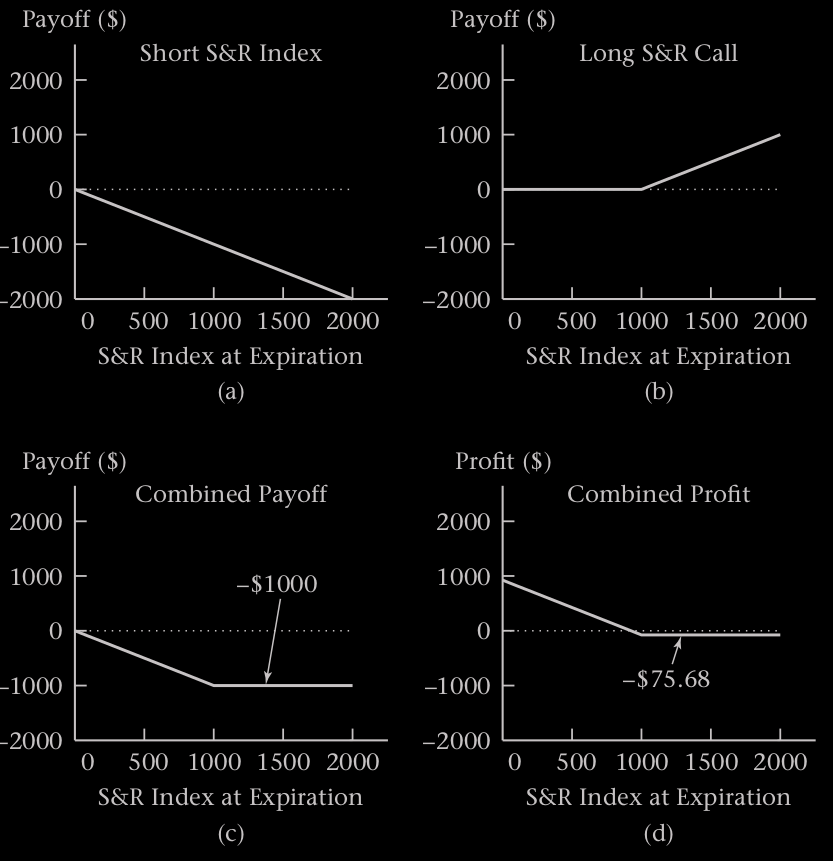
\includegraphics[scale=0.25]{figs/Figure-3-3.png}
	\end{center}
\end{frame}
%-------------- end slide -------------------------------%}}}
%-------------- start slide -------------------------------%{{{ 1
\begin{frame}[fragile,t]
	\frametitle{Selling insurance}
	\centering

	For every insurance buyer there must be an insurance seller

	\pause
	\bigskip
	\mySeparateLine
	\bigskip

	Strategies used to sell insurance
	\pause
	\bigskip

	\begin{itemize}
		\item \textcolor{magenta}{Covered writing} (\textcolor{magenta}{option overwriting} or
			\textcolor{magenta}{selling a covered call}) is writing an option when there is a corresponding long position in the
			underlying asset.

			\bigskip
		\item \textcolor{magenta}{Naked writing} is writing an option when the writer does not have a
			position in the asset.
	\end{itemize}
\end{frame}
%-------------- end slide -------------------------------%}}}
%-------------- start slide -------------------------------%{{{ 1
\begin{frame}[fragile]
\begin{center}

	\begin{minipage}{0.6\textwidth}
		\centering

		\textcolor{magenta}{Covered call writing}
		\bigskip

		Long position of the asset  + Sell a \textcolor{magenta}{call} option
	\end{minipage}
	$ \quad  \sim$
	\begin{minipage}{0.3\textwidth}
		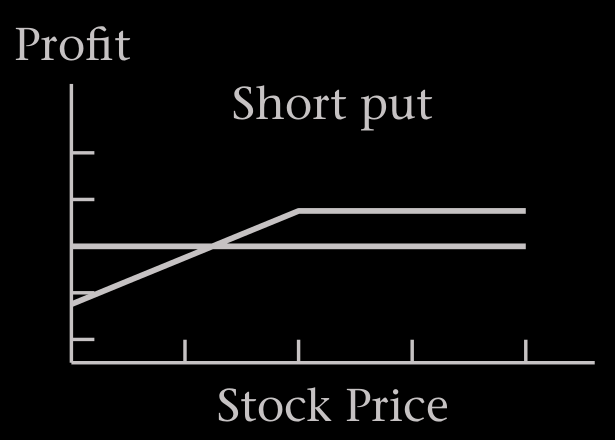
\includegraphics[scale=0.15]{figs/Short-put.png}
	\end{minipage}

	\mySeparateLine
	\bigskip

	\begin{minipage}{0.6\textwidth}
		\centering

		\textcolor{cyan}{Covered put writing}
		\bigskip

		Short position of the asset  + Sell a \textcolor{cyan}{put} option
	\end{minipage}
	$ \quad  \sim$
	\begin{minipage}{0.3\textwidth}
		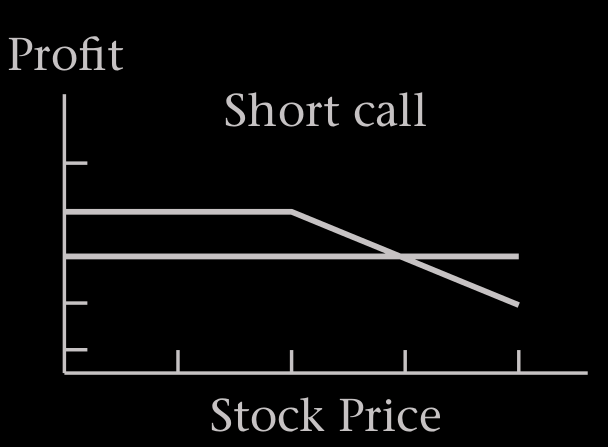
\includegraphics[scale=0.15]{figs/Short-call.png}
	\end{minipage}

\end{center}
\end{frame}
%-------------- end slide -------------------------------%}}}
%-------------- start slide -------------------------------%{{{ 1
\begin{frame}[fragile,t]
	\frametitle{Covered call writing}

	\begin{myexample}
		Under the following scenario, compute the combined profit for \underline{writing a
		\textcolor{magenta}{covered call}}
		for S\&R index.
		\begin{center}
			\renewcommand{\arraystretch}{1.2}
			\begin{tabular}{|c|c|}
				\hline
				index price today                                         & \$1,000  \\
				6-month interest rate                                     & 2\%      \\
				premium for 1000-strike 6-month \textcolor{magenta}{call} & \$93.809 \\ \hline
				% premium for 1000-strike 6-month \textcolor{cyan}{put} & \$74.201 \\ \hline
				index price at expiration                                 & \$1,100  \\ \hline
			\end{tabular}
		\end{center}
	\end{myexample}
	\vfill
	\pause
	\begin{mysol}
		\begin{align*}
			\underbrace{\$1,100 - \$1,000 \times 1.02}_{\text{profit on S\&R index}} +
			\underbrace{\$1,000-\$1,100 +\$93.809 \times 1.02}_{\text{profit on written call}} = \$75.68.
		\end{align*}
		\myEnd
	\end{mysol}
\end{frame}
%-------------- end slide -------------------------------%}}}
%-------------- start slide -------------------------------%{{{ 1
\begin{frame}[fragile]
	\begin{center}
		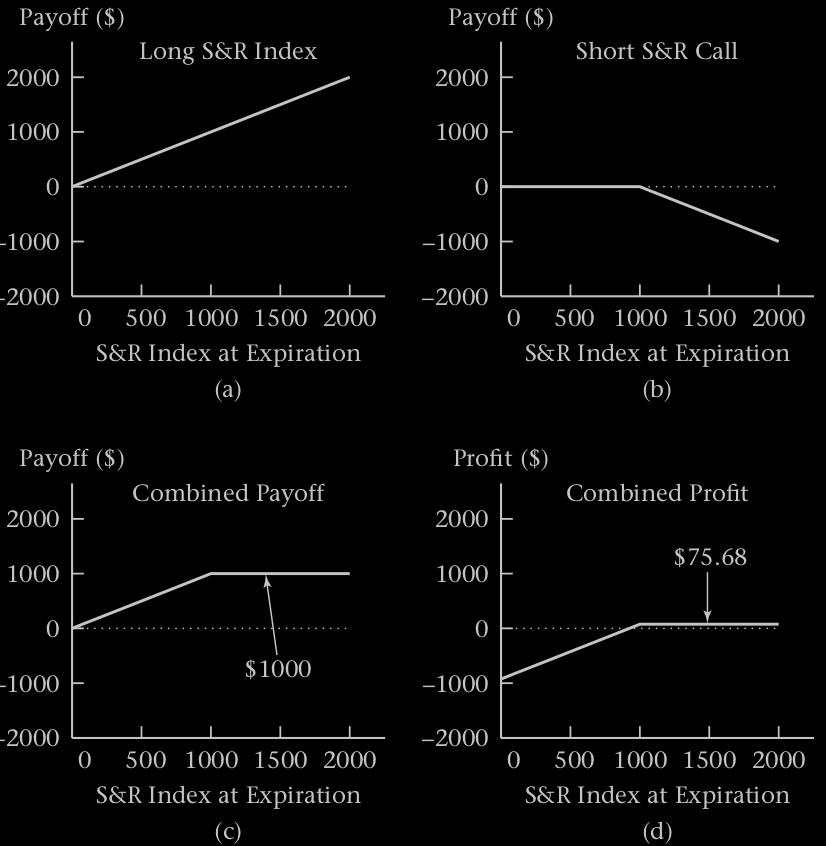
\includegraphics[scale=0.25]{figs/Figure-3-4.png}
	\end{center}
\end{frame}
%-------------- end slide -------------------------------%}}}
%-------------- start slide -------------------------------%{{{ 1
\begin{frame}[fragile,t]
	\frametitle{Covered put writing}
	\begin{myexample}
		Under the following scenario, compute the combined profit for \underline{writing a
		\textcolor{cyan}{covered put}}
		for S\&R index.
		\begin{center}
			\renewcommand{\arraystretch}{1.2}
			\begin{tabular}{|c|c|}
				\hline
				index price today                                     & \$1,000  \\
				6-month interest rate                                 & 2\%      \\
				% premium for 1000-strike 6-month \textcolor{magenta}{call} & \$93.809 \\ \hline
				premium for 1000-strike 6-month \textcolor{cyan}{put} & \$74.201 \\ \hline
				index price at expiration                             & \$900  \\ \hline
			\end{tabular}
		\end{center}
	\end{myexample}
	\vfill
	\pause
	\begin{mysol}
		\begin{align*}
			\underbrace{\$1,000 \times 1.02 - \$900}_{\text{profit on selling S\&R index}} +
			\underbrace{\$900-\$1,000 +\$74.201 \times 1.02}_{\text{profit on written put}} = \$95.685.
		\end{align*}
		\myEnd
	\end{mysol}
\end{frame}
%-------------- end slide -------------------------------%}}}
%-------------- start slide -------------------------------%{{{ 1
\begin{frame}[fragile]
	\begin{center}
		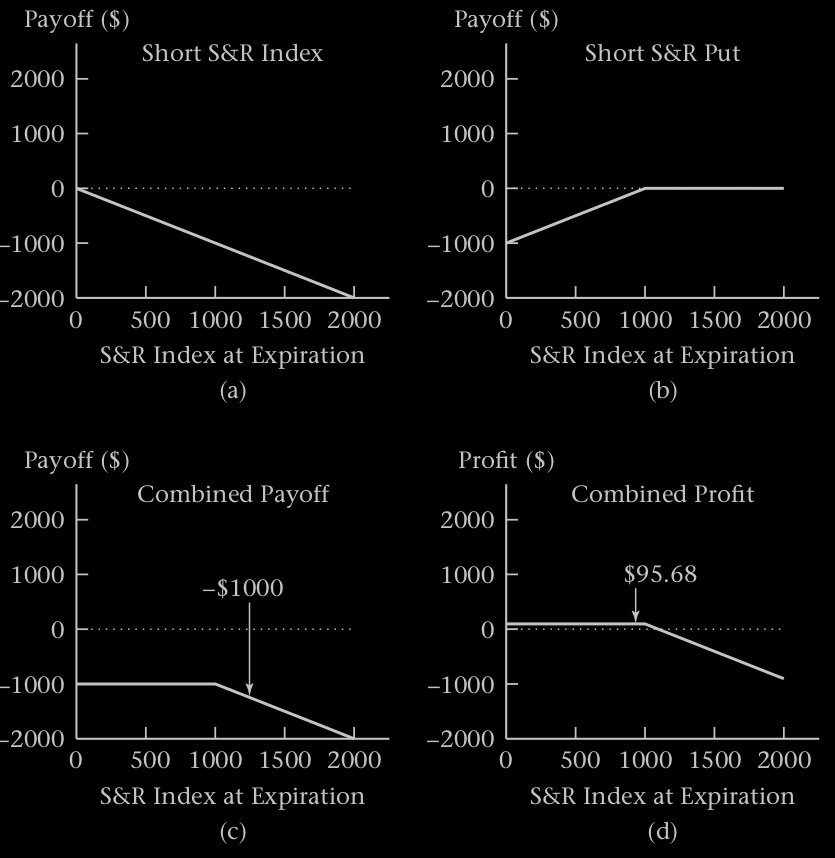
\includegraphics[scale=0.25]{figs/Figure-3-5.png}
	\end{center}
\end{frame}
%-------------- end slide -------------------------------%}}}

\def\mySecNum{3.2}
\mySection{\mySecNum~Put-call parity}
%-------------- start slide -------------------------------%{{{ 1
\begin{frame}[fragile]
\begin{center}
	It is possible to \underline{mimic a long forward position} on an asset by\\
	\bigskip

	buying a call + selling a put,\\

	\bigskip
	with each option having the same strike price and expiration time.\\

	\begin{align*}
		|  |
	\end{align*}

	\bigskip
	A synthetic forward
\end{center}
\end{frame}
%-------------- end slide -------------------------------%}}}
%-------------- start slide -------------------------------%{{{ 1
\begin{frame}[fragile,t]
\begin{myexample}
	\label{E:3-1-0}
	Working with the S\&R index. Suppose that

	\begin{center}
		\renewcommand{\arraystretch}{1.2}
		\begin{tabular}{|c|c|}
			\hline
			% index price today                                         & \$1,000  \\
			6-month interest rate                                     & 2\%      \\
			premium for 1000-strike 6-month \textcolor{magenta}{call} & \$93.809 \\
			premium for 1000-strike 6-month \textcolor{cyan}{put}     & \$74.201 \\ \hline
		\end{tabular}
	\end{center}

	Draw profit digram for the combined position of a purchased call with a written put, namely,
	\begin{center}
		\begin{minipage}{0.3\textwidth}
			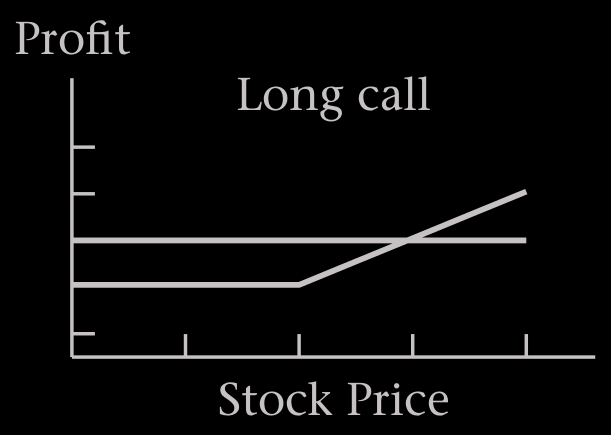
\includegraphics[scale=0.15]{figs/Long-call.png}
		\end{minipage}
		 $ \quad + \quad $
		\begin{minipage}{0.3\textwidth}
			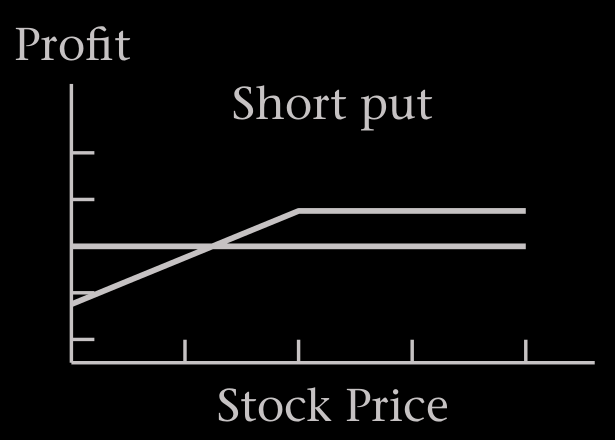
\includegraphics[scale=0.15]{figs/Short-put.png}
		\end{minipage}
	\end{center}
\end{myexample}
\end{frame}
%-------------- end slide -------------------------------%}}}
%-------------- start slide -------------------------------%{{{ 1
\begin{frame}[fragile,t]
	\begin{mysol}
		\begin{center}
			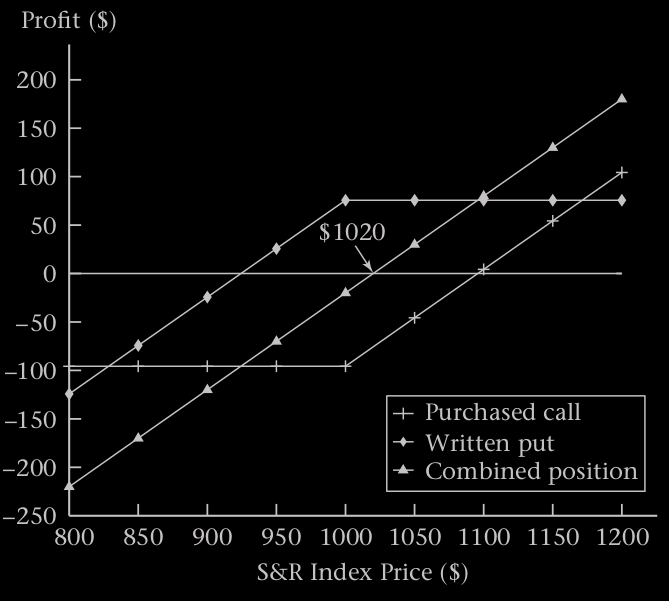
\includegraphics[scale=0.25]{figs/Figure-3-6.png}
		\end{center}
		\myEnd
	\end{mysol}
\end{frame}
%-------------- end slide -------------------------------%}}}
%-------------- start slide -------------------------------%{{{ 1
\begin{frame}[fragile,t]
	\begin{center}

		\textcolor{magenta}{A synthetic long forward contract}\\
		\bigskip

		We pay the net option premium\\[1em]
		We pay the strike price

		\bigskip
		\mySeparateLine
		\bigskip

		\textcolor{cyan}{The actual forward} \\
		\bigskip
		We pay zero premium \\[1em]
		We pay the forward price

\end{center}
\end{frame}
%-------------- end slide -------------------------------%}}}
%-------------- start slide -------------------------------%{{{ 1
\begin{frame}[fragile,t]
\begin{center}
	\textcolor{magenta}{\bf Basic Assumption}\\[1em]
	\bigskip

	The net cost of buying the index using options \\
	\bigskip

	must equal \\
	\bigskip

	the net cost of buying the index using a forward contract.

	\bigskip
	\bigskip
	\bigskip

	\pause
	\textcolor{cyan}{\bf \large NO ARBITRAGE!}

\end{center}
\end{frame}
%-------------- end slide -------------------------------%}}}
%-------------- start slide -------------------------------%{{{ 1
\begin{frame}[fragile]
\begin{center}
	\textcolor{magenta}{\bf The Put-Call parity equation}

	\begin{align*}
		\text{Call}(K,T) - \text{Put}(K,T) = \text{PV}\left(F_{0,T}-K\right)
	\end{align*}
	\pause
	\begin{itemize}
		\item $K$: strike price
		\item $T$: expiration date
		\item $\text{Call}(\cdot,\circ)$: the premium for call.
		\item $\text{Put}(\cdot,\circ)$: the premium for put.
		\item $F_{0,T}$: the forward price at time $T$ if one enters at time $0$ into a long forward position.
		\item $\text{PV}(\cdot)$: the present value function.
	\end{itemize}
\end{center}
\end{frame}
%-------------- end slide -------------------------------%}}}
%-------------- start slide -------------------------------%{{{ 1
\begin{frame}[fragile,t]
\begin{myexample}
	Check	Example \myref{E:3-1-0} to see if the put-call parity equation is satisfied.
\end{myexample}
\bigskip
\pause
\begin{mysol}
	We need to check:
	\begin{align*}
		\$93.809 - \$74.201 \stackrel{?}{=} \text{PV}(\$1,000 \times 1.02- \$1,000)
	\end{align*}
	\pause
	Clearly, $\text{LHS}=\$19.61$. \pause On the other hand, the RHS is equal to
	\begin{align*}
		\text{PV}(\$1,000 \times 1.02- \$1,000) & = \text{PV}\left(1,000 \times (1.02-1)\right) \\
                                            & = \text{PV}\left(1,000 \times 0.02\right)     \\
                                            & = \frac{1,000 \times 0.02}{1.02}              \\
																						& = \$19.61.
	\end{align*}
	\pause
	Hence, the put-call parity equation is satisfied.\myEnd
\end{mysol}
\end{frame}
%-------------- end slide -------------------------------%}}}
%-------------- start slide -------------------------------%{{{ 1
\begin{frame}[fragile,t]
	\begin{gather*}
		\textcolor{gray}{\text{Call}(K,T) - \text{Put}(K,T) = \text{PV}\left(F_{0,T}-K\right)} \\[1em]
		\textcolor{gray}{\Updownarrow}\\[1em]
		\text{PV}\left(F_{0,T}\right) +	\text{Put}(K,T) = \text{Call}(K,T) + \text{PV}\left(K\right)
	\end{gather*}

	\bigskip
	\mySeparateLine
	\bigskip

	\begin{center}
		Buying the index and buying the put \\
		\bigskip
		generate the same payoff as\\
		\bigskip
		buying the call and buying a zero-coupon bond (i.e. lending) $\text{PV}(K)$
	\end{center}
\end{frame}
%-------------- end slide -------------------------------%}}}
%-------------- start slide -------------------------------%{{{ 1
\begin{frame}[fragile,t]
	\begin{gather*}
		\textcolor{gray}{\text{Call}(K,T) - \text{Put}(K,T) = \text{PV}\left(F_{0,T}-K\right)} \\[1em]
		\textcolor{gray}{\Updownarrow}\\[1em]
		\text{PV}\left(F_{0,T}\right) -	\text{Call}(K,T) = \text{PV}\left(K\right)-\text{Put}(K,T)
	\end{gather*}

	\bigskip
	\mySeparateLine
	\bigskip

	\begin{center}
		Writing a covered call\\
		\bigskip
		has the same profit as\\
		\bigskip
		lending $\text{PV}(K)$ and selling a put
	\end{center}
\end{frame}
%-------------- end slide -------------------------------%}}}
%-------------- start slide -------------------------------%{{{ 1
\begin{frame}[fragile,t]
	\begin{gather*}
		\textcolor{green}{\text{Call}(K,T)} - \textcolor{cyan}{\text{Put}(K,T)} =
		\textcolor{magenta}{\text{PV}\left(F_{0,T}\right)}-\textcolor{yellow}{\text{PV}\left(K\right)}
	\end{gather*}

	\bigskip
	\mySeparateLine
	\bigskip
	\begin{center}
		Revisit four positions in Section 3.1\\

		\bigskip

\renewcommand{\arraystretch}{1.2}
		\begin{tabular}{|c|c|c|}
			\hline
			 Position                         & Meaning                                                              & equivalent to                                                        \\ \hline
			 Inuring a long position (floors) & \only<2->{\textcolor{magenta}{Index} $+$ \textcolor{cyan}{Put}}      & \only<3->{\textcolor{yellow}{Bound} $+$ \textcolor{green}{Call}}     \\
			 Inuring a short position (caps)  & \only<4->{$-$\textcolor{magenta}{Index} $+$ \textcolor{green}{Call}} & \only<5->{$-$\textcolor{yellow}{Bound} $+$ \textcolor{cyan}{Put}}    \\
			 Covered call writing             & \only<6->{\textcolor{magenta}{Index} $-$ \textcolor{green}{Call}}    & \only<7->{\textcolor{yellow}{Bound} $-$ \textcolor{cyan}{Put}}       \\
			 Covered put writing              & \only<8->{$-$\textcolor{magenta}{Index} $-$ \textcolor{cyan}{Put}}   & \only<9->{$-$ \textcolor{yellow}{Bound} $-$ \textcolor{green}{Call}} \\ \hline
			 \end{tabular}

	\end{center}
\end{frame}
%-------------- end slide -------------------------------%}}}

\def\mySecNum{3.3}
\mySection{\mySecNum~Spreads and collars}
%-------------- start slide -------------------------------%{{{ 1
\begin{frame}[fragile]
\begin{center}
	It is always possible                             \\
	\bigskip
	to                                                \\
	\bigskip
	\textcolor{magenta}{lower the cost of a position} \\
	\bigskip
	by                                                \\
	\bigskip
	\textcolor{cyan}{reducing its payoff!}
\end{center}
\end{frame}
%-------------- end slide -------------------------------%}}}
%-------------- start slide -------------------------------%{{{ 1
\begin{frame}[fragile,t]
	\begin{center}
		By combining two or more options, we find many well-known strategies.

	\bigskip

	\begin{center}
		\begin{tikzpicture}[scale=1, transform shape]
			\tikzset{>=latex}
			\draw[thick,->] (-0.3,0.3) -- (7,0.3);
			\draw[thick,->] (0,0) -- (0,6.5);
			\node (LC) at (2,2) {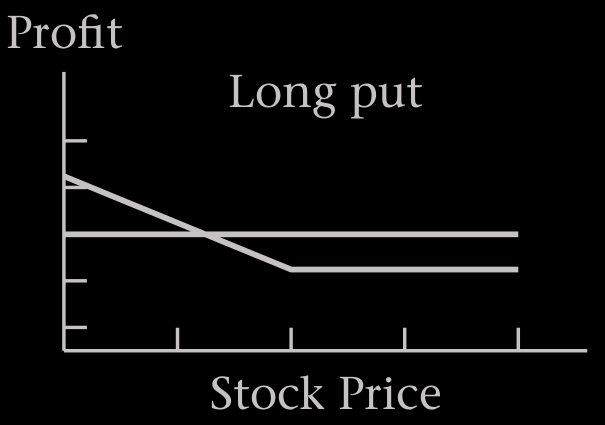
\includegraphics[scale=0.15]{figs/Long-put.png}};
			\node (LC) at (2,5) {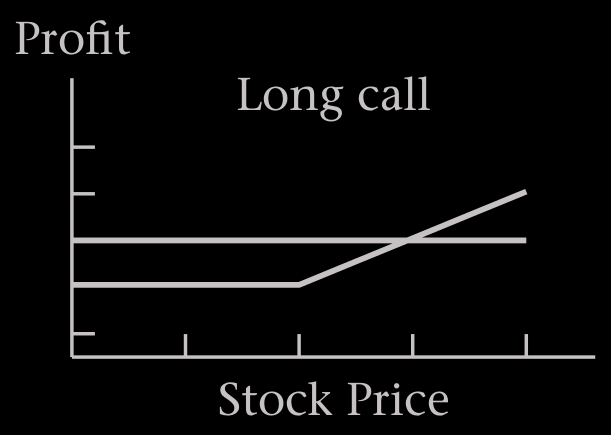
\includegraphics[scale=0.15]{figs/Long-call.png}};
			\node (LC) at (5,2) {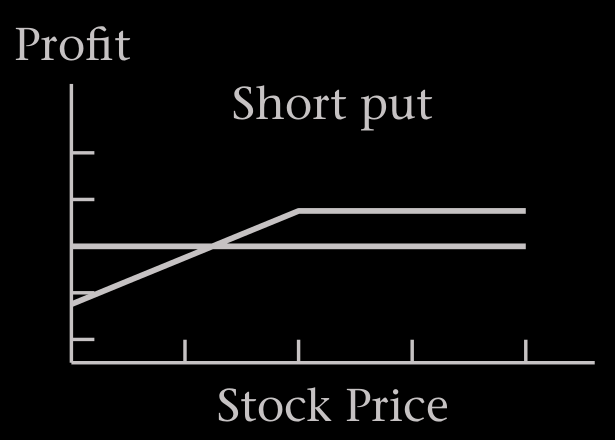
\includegraphics[scale=0.15]{figs/Short-put.png}};
			\node (LC) at (5,5) {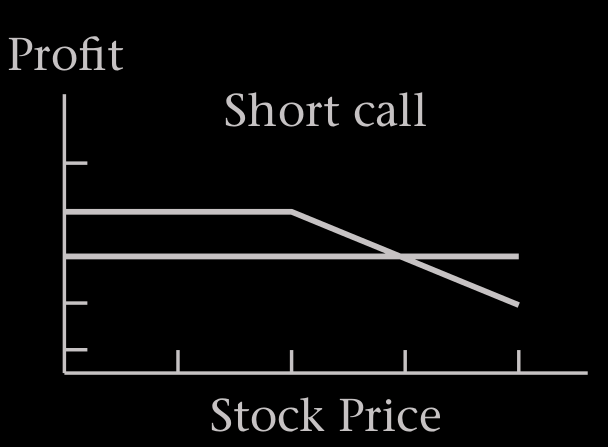
\includegraphics[scale=0.15]{figs/Short-call.png}};
			\draw[thick] (2,0.5) -- ++ (0,-0.5) node [below] {Long};
			\draw[thick] (5,0.5) -- ++ (0,-0.5) node [below] {Short};
			\draw[thick] (0.2,5) -- ++ (-0.5,0) node [left] {Call};
			\draw[thick] (0.2,2) -- ++ (-0.5,0) node [left] {Put};
		\end{tikzpicture}
	\end{center}
	\end{center}
\end{frame}
%-------------- end slide -------------------------------%}}}
%-------------- start slide -------------------------------%{{{ 1
\begin{frame}[fragile]
	\begin{center}
	\begin{center}
		\begin{tikzpicture}[scale=1, transform shape]
			\tikzset{>=latex}
			\draw[thick,->] (-0.3,0.3) -- (7,0.3);
			\draw[thick,->] (0,0) -- (0,6.5);
			% \node (LC) at (2,2) {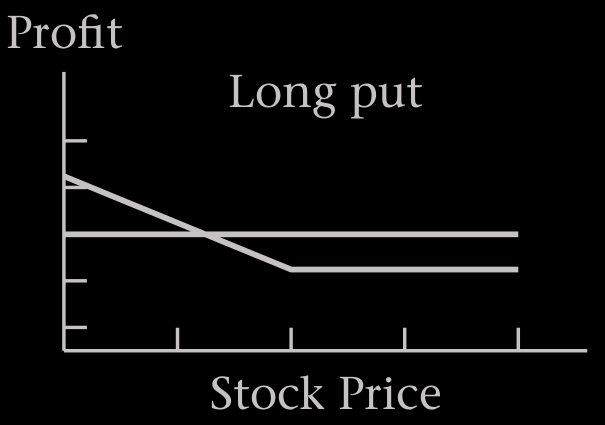
\includegraphics[scale=0.15]{figs/Long-put.png}};
			% \node (LC) at (2,5) {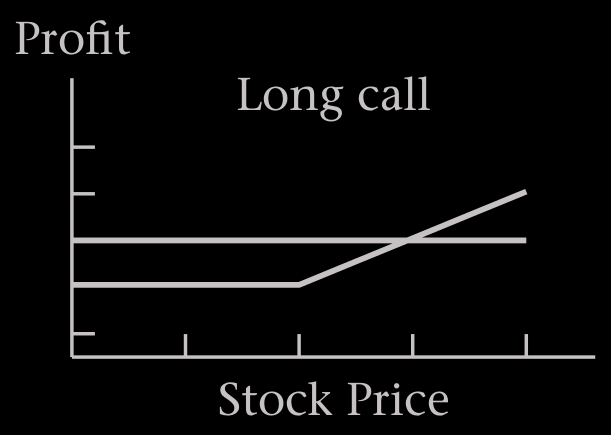
\includegraphics[scale=0.15]{figs/Long-call.png}};
			% \node (LC) at (5,2) {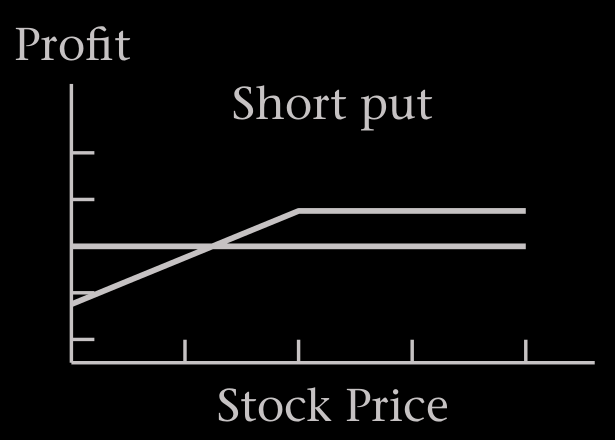
\includegraphics[scale=0.15]{figs/Short-put.png}};
			% \node (LC) at (5,5) {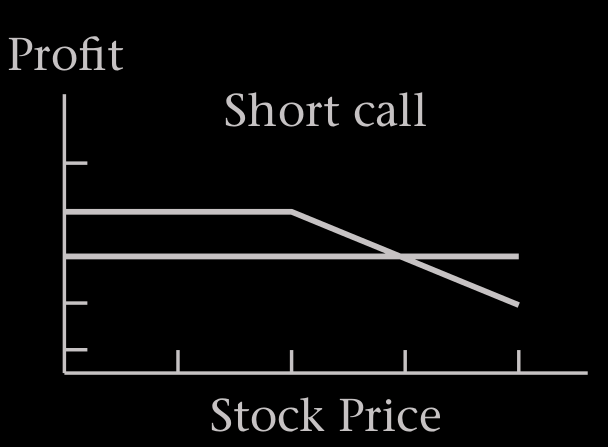
\includegraphics[scale=0.15]{figs/Short-call.png}};
			\draw[thick,red] (0.5,3.5) -- (1.5,0.5)  node [midway,above, sloped] {long} -- (3,0.5) node [midway,above, sloped, red] {put};
			\draw[thick,green] (3,0.5) -- (4,3.5) node [midway, above, sloped] {short} -- (6.5,3.5) node [midway, above, sloped] {put};
			\draw[thick,cyan] (6.5,3.5) -- (5.5,6.5) node [midway, above, sloped] {call} -- (4,6.5) node [midway, above, sloped] {short};
			\draw[thick,magenta] (4,6.5) -- (3,3.5) node [midway, above, sloped] {call} -- (0.5,3.5) node [midway, above, sloped] {long};

			\draw[thick] (2,0.5) -- ++ (0,-0.5) node [below] {Long};
			\draw[thick] (5,0.5) -- ++ (0,-0.5) node [below] {Short};
			\draw[thick] (0.2,5) -- ++ (-0.5,0) node [left] {Call};
			\draw[thick] (0.2,2) -- ++ (-0.5,0) node [left] {Put};
		\end{tikzpicture}
	\end{center}
	\end{center}
\end{frame}
%-------------- end slide -------------------------------%}}}
%-------------- start slide -------------------------------%{{{ 1
\begin{frame}[fragile,t]

	An \textcolor{magenta}{option spread} is a position consisting of only calls or only puts, in
	which some options are purchased and some written.
	\bigskip

	\begin{itemize}
		\item Bull and bear spreads
			\bigskip
		\item Box spreads
			\bigskip
		\item Ratio spreads
			\bigskip
		\item Collars
	\end{itemize}


\end{frame}
%-------------- end slide -------------------------------%}}}
%-------------- start slide -------------------------------%{{{ 1
\begin{frame}[fragile,t]
	\frametitle{Example for this section}
	\begin{center}
		Black-Scholes option prices \\
		\begin{align*}
			\text{Stock price}                     & = \$40   \\
			\text{Volatility}                      & = 30\%   \\
			\text{Effective annual risk-free rate} & = 8.33\% \\
			\text{Dividend yield} & = \$0 \\
			\text{Expriation days} & = 91~\text{days}
		\end{align*}

		\bigskip
		\renewcommand{\arraystretch}{1.2}
		\begin{tabular}{ccc}
			\hline
			Strike & Call & Put  \\
			\hline
			35     & 6.13 & 0.44 \\
			40     & 2.78 & 1.99 \\
			45     & 0.97 & 5.08 \\
		\end{tabular}
		\end{center}
\end{frame}
%-------------- end slide -------------------------------%}}}
%-------------- start slide -------------------------------%{{{ 1
\begin{frame}[fragile,t]
	\frametitle{Bull and bear spreads}

	\bigskip
	A position in which you buy a call and sell  an otherwise identical call with a higher strike price
	is an example of a \textcolor{magenta}{bull spread}. Bull spreads can also be constructed using
	puts.

	\bigskip
	The opposite of a bull spread is a \textcolor{magenta}{bear spread}.

\end{frame}
%-------------- end slide -------------------------------%}}}
%-------------- start slide -------------------------------%{{{ 1
\begin{frame}[fragile]
	\begin{center}
		\begin{tikzpicture}[scale=1, transform shape]
			\tikzset{>=latex}
			\draw[->, thick] (-4,0) -- (4,0) node [right] {Strike price};
			\draw[thick] (-2,0.3) -- ++(0,-0.6) node [below] {low};
			\draw[thick] (2,-0.3) -- ++(0,0.6) node [above] {high};
			\pause
			\node at (0,4) {\textcolor{magenta}{Bull spread}};

			\pause
			% \draw (-1.9,2) circle (1.2);
			\node at  (-2.5,2.5) {Long};
			\node at  (-1.5,2.5) {Call};
			\node at  (-2.5,1.5) {Short};
			\node at  (-1.5,1.5) {Put};

			\pause
			% \draw (1,1) rectangle (3,3);
			\node at  (1.5,2.5) {Short};
			\node at  (2.5,2.5) {Call};
			\node at  (1.5,1.5) {Long};
			\node at  (2.5,1.5) {Put};
			\node at (0,2) {$+$};

			\pause
			\node at (0,-4) {\textcolor{cyan}{Bear spread}};

			\pause
			% \draw (-1,-1) rectangle (-3,-3);
			\node at  (-2.5,-1.5) {Long};
			\node at  (-1.5,-1.5) {Put};
			\node at  (-2.5,-2.5) {Short};
			\node at  (-1.5,-2.5) {Call};

			\pause
			% \draw (1.9,-2) circle (1.2);
			\node at  (1.5,-1.5) {Short};
			\node at  (2.5,-1.5) {Put};
			\node at  (1.5,-2.5) {Long};
			\node at  (2.5,-2.5) {Call};

			\node at (0,-2) {$+$};

			\pause
			\draw[magenta, thick] (-3,0.3) -- (-2,0.3) -- (2,4.3) -- (3,4.3);
			\draw[cyan, thick] (-3,-0.3) -- (-2,-0.3) -- (2,-4.3) -- (3,-4.3);
			\draw[dotted] (2,4.5) -- ++ (0,-9);
			\draw[dotted] (-2,0.5) -- ++ (0,-1);
			\draw[thick,->,magenta] (-3.5,0.3) -- ++ (0, 4) node [midway,sloped,above] {Profit};
			\draw[thick,->,cyan] (-3.5,-4.3) -- ++ (0, 4) node [midway,sloped,above] {Profit};
		\end{tikzpicture}
	\end{center}
\end{frame}
%-------------- end slide -------------------------------%}}}
%-------------- start slide -------------------------------%{{{ 1
\begin{frame}[fragile,t]
	\begin{myexample}
		Draw profit diagram for a 40-45	bull spread, namely, buying a 40-strike call and selling
		a 45-strike call.
	\end{myexample}
	\pause
	\begin{mysol}\phantom{a}\\
		\begin{center}
			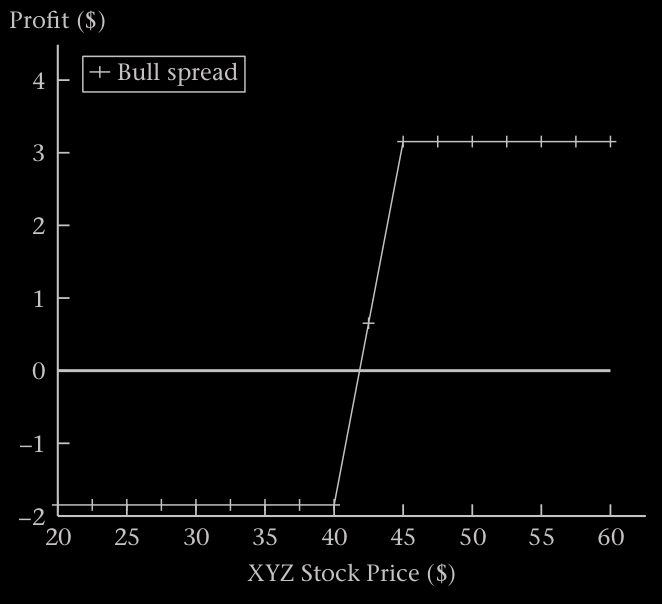
\includegraphics[scale=0.2]{figs/Figure-3-7.png}
		\end{center}

		We only need to determine the two levels.
	\end{mysol}
\end{frame}
%-------------- end slide -------------------------------%}}}
%-------------- start slide -------------------------------%{{{ 1
\begin{frame}[fragile,t]
	\begin{mysol}[(Continued)]\\
		\bigskip

		(a)	 Suppose that the index price is \$ 30 at the expiration:
		\begin{align*}
			\left(\$ 2.78 - \$ 0.97 \right) \times (1+0.0833)^{1/4} = \textcolor{magenta}{\$ 1.85}.
		\end{align*}
		\bigskip \pause

		(b) Suppose that the index price is \$50 at the expiration:
		\begin{align*}
			(\$50 - \$40) - (\$ 40 - \$ 45) - \textcolor{magenta}{\$ 1.85} = \$ 3.15.
		\end{align*}
		\myEnd
	\end{mysol}
\end{frame}
%-------------- end slide -------------------------------%}}}
%-------------- start slide -------------------------------%{{{ 1
\begin{frame}[fragile,t]
	\frametitle{Box spreads}

	A \textcolor{magenta}{\bf box spread} is accomplished by using options to create
	\textcolor{magenta}{a synthetic long forward} at one price and \textcolor{cyan}{a synthetic short
	forward} at a different price.
	\bigskip

	This strategy guarantees a cash flow in the future.
	\bigskip

	Hence, it is an option spread that is purely a means of borrowing or lending money. It is costly
	but has no stock price risk.
\end{frame}
%-------------- end slide -------------------------------%}}}
%-------------- start slide -------------------------------%{{{ 1
\begin{frame}[fragile,t]
\begin{myexample}
	Suppose we simultaneously enter into the following two transactions:
	\begin{enumerate}
		\item Buy a 40-strike call and sell a 40-strike put.
		\item Sell a 45-strike call and buy a 45-strike put.
	\end{enumerate}
	\pause
	Explain why there is no free lunch. Draw the profit diagram.
\end{myexample}
\bigskip
\pause
\begin{mysol}
	The profit is
	\begin{align*}
		5 + \underbrace{(1.99-2.78)\times (1.0833)^{1/4}}_{\text{Synthetic long forward}}
		+ \underbrace{(0.97-5.08)\times (1.0833)^{1/4}}_{\text{Synthetic short forward}}
		= \$ 0.0099851.
	\end{align*}
  %
	% 5 + (1.99-2.78)*(1.0833)**0.25 +(0.97-5.08)*(1.0833)**0.25
  %
	\myEnd
\end{mysol}
\end{frame}
%-------------- end slide -------------------------------%}}}
%-------------- start slide -------------------------------%{{{ 1
\begin{frame}[fragile]
\begin{center}
	\begin{tikzpicture}[scale=1, transform shape]
		\tikzset{>=latex}
		\node[] (a) at (-2,+1) {Buy  a \$40-strike call}; \node[] (a) at (+2,+1) {Sell a \$40-strike put};
		\node[] (a) at (-2,-1) {Sell a \$45-strike call}; \node[] (a) at (+2,-1) {Buy  a \$45-strike put};
		\node[] (b) at (-2,-3) {Bull spread}; \draw [->] (b) -- ++(0,1.2);
		\node[] (b) at (+2,-3) {Bear spread}; \draw [->] (b) -- ++(0,1.2);
		\node[] (c) at (6,1) {Synthetic long forward};
		\node[] (c) at (+6,-1) {Synthetic short forward};
		\draw (-4,-1.5) rectangle (4,1.5);
	\end{tikzpicture}
\end{center}
\end{frame}
%-------------- end slide -------------------------------%}}}
%-------------- start slide -------------------------------%{{{ 1
\begin{frame}[fragile,t]
	\frametitle{Ratio spreads}

	A \textcolor{magenta}{\bf ratio spread} is constructed by buying m options at one strike and
	selling n options at a different strike, with all options having the same type (call or put), same
	time to maturity, and same underlying asset.
	\bigskip

	\begin{center}
		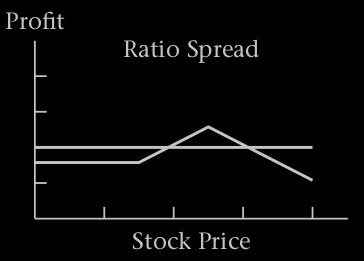
\includegraphics[scale=0.3]{figs/Profit_Ratio_Spread.png}
	\end{center}

\end{frame}
%-------------- end slide -------------------------------%}}}
%-------------- start slide -------------------------------%{{{ 1
\begin{frame}[fragile,t]
	\begin{myexample}[(Problem 3.15)]
	Compute profit diagrams for the following ratio spreads:
	\begin{itemize}
		\item[a] Buy 950-strike call, sell two 1050-strike calls.
		\item[b] Buy two 950-strike calls, sell three 1050-strike calls.
		\item[c] Consider buying n 950-strike calls and selling m 1050-strike calls so that the premium of the position is zero. Considering your analysis in (a) and (b), what can you say about n/m? What exact ratio gives you a zero premium?
	\end{itemize}
	\begin{center}
\renewcommand{\arraystretch}{1.2}
		\begin{tabular}{|c|c|c|}
		\hline
		Strike & Call      & Put      \\ \hline
		\$950  & \$120.405 & \$51.777 \\
		1000   & 93.809    & 74.201   \\
		1020   & 84.470    & 84.470   \\
		1050   & 71.802    & 101.214  \\
		1107   & 51.873    & 137.167  \\ \hline
		\end{tabular}
	\end{center}
	\end{myexample}
	\pause
	\begin{mysol}
		\textcolor{gray}{...}	\myEnd
	\end{mysol}
\end{frame}
%-------------- end slide -------------------------------%}}}
%-------------- start slide -------------------------------%{{{ 1
\begin{frame}[fragile,t]
	\frametitle{Collars}

	A \textcolor{magenta}{\bf collar} is the purchase of a put option and the sale of a call option with
	a higher strike price, with both options having the same underlying asset and having the same
	expiration date.

	\bigskip

	If the position is reversed, i.e., sale of a put and purchase of a call, the collar is written.

	\bigskip

	The \textcolor{magenta}{\bf collar width} is the difference between the call and put strikes.
\end{frame}
%-------------- end slide -------------------------------%}}}
%-------------- start slide -------------------------------%{{{ 1
\begin{frame}[fragile,t]
\begin{myexample}
 	Draw the profit diagram for a purchased collar:
	\begin{align*}
		\text{selling a 45-strike call} + \text{buying a 40-strike put}.
	\end{align*}
\end{myexample}
\pause
\bigskip
\begin{mysol}
	One can easily draw the profit graph. We only need to determine the level when the curve is flat. Hence, 
	suppose the price is \$43. Then the profit is
	\begin{align*}
		(0.97-1.99) \times (1.083)^{1/4} = -\$1.0405.
	\end{align*}
	\bigskip

	\begin{center}
		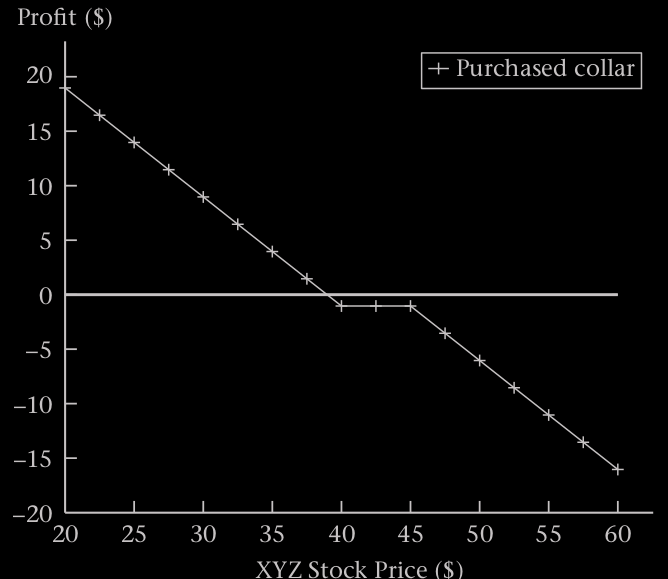
\includegraphics[scale=0.2]{figs/Figure-3-8.png}
	\end{center}
	\myEnd
\end{mysol}
\end{frame}
%-------------- end slide -------------------------------%}}}
%-------------- start slide -------------------------------%{{{ 1
\begin{frame}[fragile,t]
It is possible to find strike prices for the put and call such that the two premiums exactly offset one another. This
position is called a \textcolor{magenta}{\bf zero-cost collar}.
\end{frame}
%-------------- end slide -------------------------------%}}}
%-------------- start slide -------------------------------%{{{ 1
\begin{frame}[fragile,t]
	\begin{myexample}
		Consider XYZ:
		\begin{center}
			\renewcommand{\arraystretch}{1.2}
			\begin{tabular}{ccc}
				\hline
				Strike                     & Call                      & Put                      \\
				\hline
				35                         & 6.13                      & 0.44                     \\
				40                         & 2.78                      & \textcolor{cyan}{1.99}   \\
				\textcolor{magenta}{41.72} & \textcolor{magenta}{1.99} & \textcolor{magenta}{---} \\
				45                         & 0.97                      & 5.08                     \\
			\end{tabular}
		\end{center}
		where we need to use \textcolor{red}{Black-Scholes formula} to find out the strike price, which is \textcolor{magenta}{41.72},
		when the put premium is \textcolor{magenta}{\$1.99}.
		This gives a zero-cost collar.
		% \begin{align*}
		% 	\text{buying XYZ at \$40} + \text{buying a 40-strike put} + \text{selling a 41.72-strike call}
		% \end{align*}
		% Draw the profit diagram.
	\end{myexample}
	% \pause
	% \bigskip
	% \begin{mysol}
	% 	\textcolor{gray}{Check book p. 77.} \myEnd
	% \end{mysol}
\end{frame}
%-------------- end slide -------------------------------%}}}

\def\mySecNum{3.4}
\mySection{\mySecNum~Speculating on volatility}
%-------------- start slide -------------------------------% {{{
\begin{frame}[fragile,t]
	\begin{center}

		\begin{minipage}{0.37\textwidth}
			\textcolor{magenta}{Directional positions}
			\pause
			\begin{itemize}
				\item Bull spread
				\item Bear spread
				\item Collars
				\item Box spreads
			\end{itemize}
		\end{minipage}

		\pause
		\bigskip
		\mySeparateLine
		\bigskip

		\begin{minipage}{0.37\textwidth}
			\textcolor{cyan}{Nondirectional positions}
			\pause
			\begin{itemize}
				\item Straddles
				\item Strangle
				\item Butterfly spread
			\end{itemize}
		\end{minipage}
		\bigskip

		\pause
		Investors who do not care whether the stock goes up or down, \\
		but only \alert{how much it moves}.                          \\
		\bigskip

		Investors are speculating on                                 \\
		\bigskip

		\alert{\huge volatility}
	\end{center}
\end{frame}
%-------------- end slide -------------------------------%}}}
%-------------- start slide -------------------------------%{{{ 1
\begin{frame}[fragile,t]
	\frametitle{Example for this section}
	\begin{center}
		Black-Scholes option prices \\
		\begin{align*}
			\text{Stock price}                     & = \$40   \\
			\text{Volatility}                      & = 30\%   \\
			\text{Effective annual risk-free rate} & = 8.33\% \\
			\text{Dividend yield} & = \$0 \\
			\text{Expriation days} & = 91~\text{days}
		\end{align*}

		\bigskip
		\renewcommand{\arraystretch}{1.2}
		\begin{tabular}{ccc}
			\hline
			Strike & Call & Put  \\
			\hline
			35     & 6.13 & 0.44 \\
			40     & 2.78 & 1.99 \\
			45     & 0.97 & 5.08 \\
		\end{tabular}
		\end{center}
\end{frame}
%-------------- end slide -------------------------------%}}}
%-------------- start slide -------------------------------%{{{ 1
\begin{frame}[fragile,t]
	\frametitle{Straddles}

	\textcolor{magenta}{\bf Straddle} is the strategy of buying a call and a put with the same strike
	price and time to expiration.
	\bigskip

	A straddle is a bet that \textcolor{red}{volatility will be high} relative to the market’s assessment
	\bigskip

	\begin{center}
		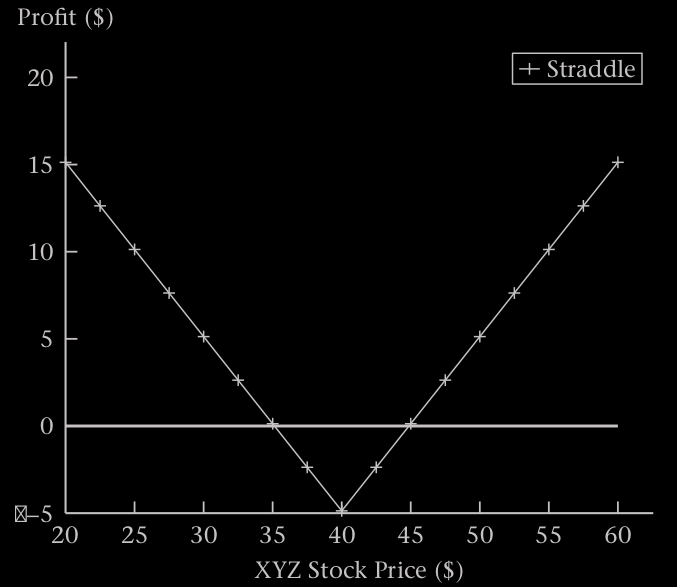
\includegraphics[scale=0.25]{figs/Figure-3-10.png}
	\end{center}
\end{frame}
%-------------- end slide -------------------------------%}}}
%-------------- start slide -------------------------------%{{{ 1
\begin{frame}[fragile,t]
\begin{myexample}
	Draw the profit graph for a \$40=strike straddle.
\end{myexample}
\pause
\bigskip
\begin{mysol}
	We only need to determine the tip of the graph:
	\begin{align*}
		-(2.78+1.99) \times (1+0.083)^{1/4} = -\$ 4.8660.
	\end{align*}
	Hence,

	\begin{center}
		\begin{tikzpicture}[scale=1, transform shape]
			\tikzset{>=latex}
			\draw[->] (-0.5,0) -- (7.5,0) node [below] {Stock price};
			\draw[->] (0,-1) -- (0,0.1) node [above] {\$0} -- (0,4) node [above] {Profit};
			\draw (0,3) -- (3.5,-0.5) -- (7,3);
			\draw (0.1,-0.5) -- ++(-0.2,0) node [left] {-\$4.866};
			\draw (3,0.1) -- ++(0,-0.2) node [below] {\$35.13};
			\draw (4,0.1) -- ++(0,-0.2) node [below] {\$44.87};
			\draw (3.5,-0.1) -- ++(0,0.2) node [above] {\$40};
			\draw (1.725,-0.1) -- ++(0,0.2) node [above] {\$20};
			\draw (5.225,-0.1) -- ++(0,0.2) node [above] {\$60};
			\draw (7,-0.1) -- ++(0,0.2) node [above] {\$80};
			\draw (0.1,3) -- ++(-0.2,0) node [left] {\$35.13};
			\draw [dashed, ->] (3.5,1.5) node[above] {Breakeven prices} -- (3,0.12);
			\draw [dashed, ->] (3.5,1.5) -- (4,0.12);
			\draw [dotted] (0,-0.5) -- ++(3.5,0);
		\end{tikzpicture}
	\end{center}
	\myEnd
\end{mysol}
\end{frame}
%-------------- end slide -------------------------------%}}}
%-------------- start slide -------------------------------%{{{ 1
\begin{frame}[fragile,t]
	\frametitle{Strangle}

	\textcolor{cyan}{\bf Strangle} is the strategy of	buying an out-of-the-money call and put with
	the same time to expiration.
	\bigskip

	\begin{center}
		A \textcolor{cyan}{strangle} can be used to reduce the high premium cost, \\
		associated with a \textcolor{magenta}{straddle}.
	\end{center}

	\vfill
	\begin{center}
		\renewcommand{\arraystretch}{1.2}
		\begin{tabular}{c|cc}
			\hline
                                    & Buying call at a strike price & Buying put at a strike price \\ \hline
			\textcolor{magenta}{Straddle} & Same                          & Same                         \\
			\textcolor{cyan}{Strangle}    & High                          & Low                          \\
			\hline
		\end{tabular}

	\end{center}
\end{frame}
%-------------- end slide -------------------------------%}}}
%-------------- start slide -------------------------------%{{{ 1
\begin{frame}[fragile,t]
	\begin{myexample}
		Draw profit diagram for 40-strike straddle and strangle composed of
		\begin{align*}
			\text{35-strike put} + \text{45-strike call}.
		\end{align*}
	\end{myexample}
	\pause
	\bigskip
	\begin{mysol}
		We know the shape of the graph and need only to determine the level of the flat part. Hence,
		suppose the stock price is \$40. Then the profit is
		\begin{align*}
			-(0.44+0.97)\times(1+0.083)^{1/4}=-\$1.4384.
		\end{align*}
		The breakeven prices are
		\begin{align*}
			45+1.4384 = \$46.4384 \quad \text{and} \quad 35-1.4384 = \$ 33.562.
		\end{align*}
	\end{mysol}
\end{frame}
%-------------- end slide -------------------------------%}}}
%-------------- start slide -------------------------------%{{{ 1
\begin{frame}[fragile,t]
	\begin{center}
		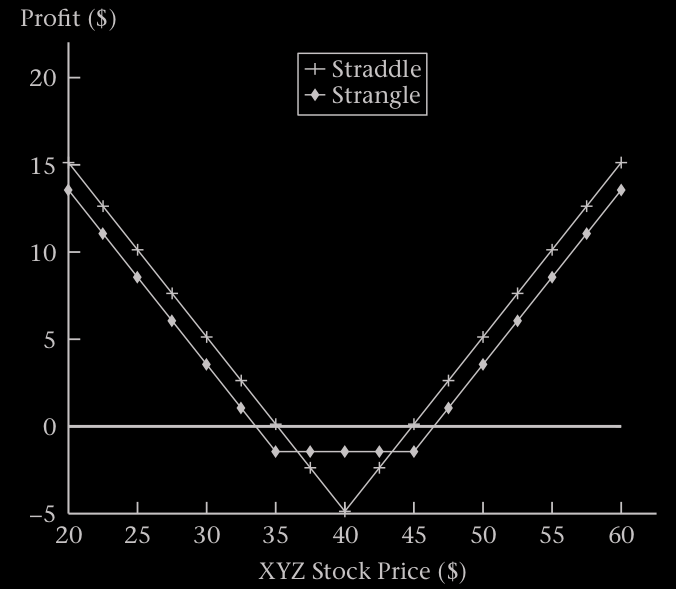
\includegraphics[scale=0.25]{figs/Figure-3-11.png}
	\end{center}
	\myEnd
\end{frame}
%-------------- end slide -------------------------------%}}}
%-------------- start slide -------------------------------% {{{
\begin{frame}[fragile,t]
	\frametitle{Written straddles}

	\textcolor{magenta}{\bf Written straddle} is the strategy of
	selling a call and put with the same strike price and time to maturity.
	\bigskip


	\begin{center}
		Unlike a purchased straddle, a written straddle is a bet that \\
		\bigskip

		\textcolor{red}{volatility will be low}
		\bigskip

		relative to the market’s assessment.
	\end{center}

	\bigskip

	\begin{center}
		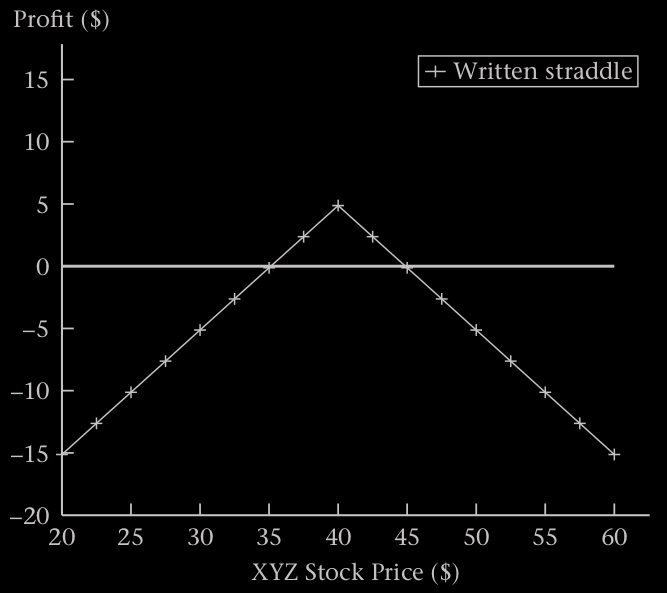
\includegraphics[scale=0.25]{figs/Figure-3-12.png}
	\end{center}
\end{frame}
%-------------- end slide -------------------------------%}}}
%-------------- start slide -------------------------------% {{{
\begin{frame}[fragile,t]
	\frametitle{Butterfly spreads}
	\begin{align*}
		\text{\textcolor{magenta}{\bf Butterfly spreads}} & = \text{Insured wri\text{en straddle}} \\
																											& = \text{\textcolor{magenta}{Written straddle}}  + \text{\textcolor{cyan}{purchased straggle}}
	\end{align*}

	\begin{center}
		A butterfly spread insures against large losses on a straddle.
		\bigskip
		\bigskip

		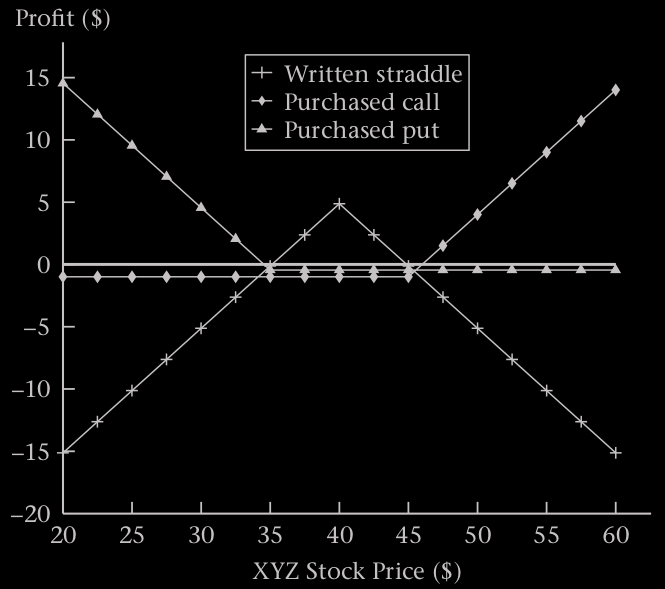
\includegraphics[scale=0.2]{figs/Figure-3-13.png}
		\quad
		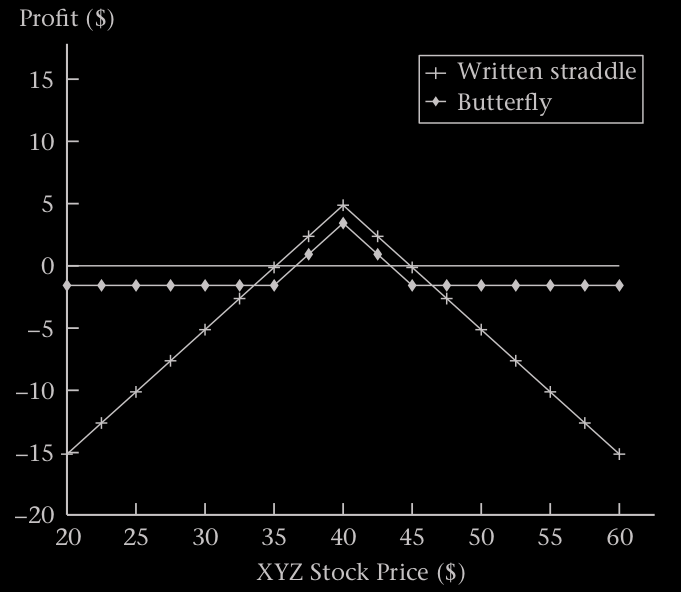
\includegraphics[scale=0.2]{figs/Figure-3-14.png}
	\end{center}
\end{frame}
%-------------- end slide -------------------------------%}}}
%-------------- start slide -------------------------------%{{{ 1
\begin{frame}[fragile,t]
\begin{myexample}
	Draw the profit graph for the butterfly spread:
	\begin{align*}
		\text{Written \$40 \textcolor{magenta}{straddle}} + \text{purchased 35-45 \textcolor{cyan}{straggle}}.
	\end{align*}
	\pause \bigskip

	\begin{mysol}
		First notice that this spread corresponds:
		\begin{center}
			\renewcommand{\arraystretch}{1.2}
			\begin{tabular}{ccc}
				\hline
				Strike & Call                              & Put                               \\
				\hline
				35     & 6.13                              & 0.44 (\textcolor{cyan}{long})     \\
				40     & 2.78 (\textcolor{magenta}{short}) & 1.99 (\textcolor{magenta}{short}) \\
				45     & 0.97 (\textcolor{cyan}{long})     & 5.08                              \\
			\end{tabular}
		\end{center}
		We know the general shape of the profit graph and need only to determine the level when the graph is flat. For this, suppose that the stock price is \$ $x<30$.
		In this case, only both puts are in the money and the profit is
		\begin{align*}
			(\textcolor{magenta}{2.78}+\textcolor{magenta}{1.99} - \textcolor{cyan}{0.44} -\textcolor{cyan}{0.97}) \times (1+0.083)^{1/4} + (35-x) + (x-40) = -\$1.5724.
		\end{align*}
	\end{mysol}
	% (2.78+1.99-0.44-0.97)*(1.083^0.25) -5
\end{myexample}
\end{frame}
%-------------- end slide -------------------------------%}}}
%-------------- start slide -------------------------------%{{{ 1
\begin{frame}[fragile,t]
	\begin{center}
			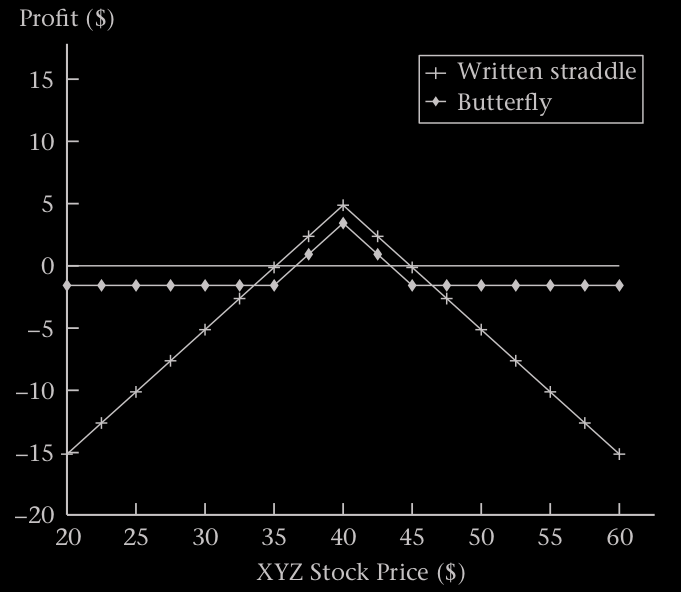
\includegraphics[scale=0.3]{figs/Figure-3-14.png}
	\end{center}
	\myEnd
\end{frame}
%-------------- end slide -------------------------------%}}}

\def\mySecNum{3.5}
\mySection{\mySecNum~Problems}
%-------------- start slide -------------------------------%{{{ 1
\begin{frame}[fragile,t]
	Problems:
	3.3,
	3.4,
	3.5,
	3.6,
	3.7,
	3.8,
	3.9,
	3.11,
	3.13,
	3.14,
	3.15,
	3.17,
	3.18.
	\\
	\bigskip

	Due Date: TBA
\end{frame}
%-------------- end slide -------------------------------%}}}

\end{document}
